\pdfminorversion=7
\documentclass[10pt]{article}
\usepackage[margin=0.85in]{geometry}
\usepackage[T1]{fontenc}
\usepackage[utf8]{inputenc}
\usepackage{lmodern}
\usepackage{amsmath,amssymb,amsthm}
\usepackage{booktabs}
\usepackage{tabularx}
\usepackage{enumitem}
\usepackage{xcolor}
\usepackage{listings}
\usepackage{graphicx}
\usepackage{tikz}
\definecolor{bpgreen}{HTML}{1CAC78}
\definecolor{bpdef}{HTML}{B0ECA3}
\definecolor{bpblue}{HTML}{1F5FD6}
\usetikzlibrary{arrows.meta,positioning,shapes.geometric}
\usepackage[colorlinks=true,linkcolor=blue!50!black,citecolor=blue!50!black,urlcolor=blue!50!black]{hyperref}

\graphicspath{{./}{report/}}

\setlist{itemsep=1.5pt,topsep=3pt}
\emergencystretch=3em
\let\origus\_
\renewcommand{\_}{\origus\allowbreak}

\newtheorem{theorem}{Theorem}
\newcommand{\N}{\mathbb{N}}
\newcommand{\Part}{\mathrm{Part}}
\newcommand{\Partrec}{\mathrm{Partrec}}
\newcommand{\TM}{\mathrm{TM0}}
\newcommand{\code}[1]{\texttt{#1}}

% ---- Auto-populated Repository & Audit Metrics ----
\newcommand{\LeanToolchain}{leanprover/lean4:v4.36.0}
\newcommand{\NModules}{8}
\newcommand{\NLines}{2{,}091}
\newcommand{\NTotalNodes}{22}
\newcommand{\NProvedNodes}{17}
\newcommand{\NDefNodes}{5}
\newcommand{\NLeanDecls}{51}
\newcommand{\NSorryAx}{0}

\lstdefinelanguage{lean}{
  morekeywords={theorem,lemma,def,structure,class,where,by,fun,let,have,exact,obtain,refine,import,namespace,end,variable,open,Nonempty,Fintype,DecidableEq,Inhabited},
  sensitive=true, morecomment=[l]{--}, morecomment=[s]{/-}{-/}, morestring=[b]"}
\lstset{language=lean,basicstyle=\ttfamily\scriptsize,keywordstyle=\bfseries\color{blue!50!black},
  commentstyle=\itshape\color{gray},columns=fullflexible,keepspaces=true,frame=single,framerule=0.3pt,
  xleftmargin=4pt,xrightmargin=4pt,breaklines=true,
  literate={→}{{$\to$}}1 {∀}{{$\forall$}}1 {∃}{{$\exists$}}1 {¬}{{$\neg$}}1 {≤}{{$\le$}}1 {ℕ}{{$\mathbb{N}$}}1
           {⟨}{{$\langle$}}1 {⟩}{{$\rangle$}}1 {∧}{{$\wedge$}}1 {∘}{{$\circ$}}1 {↔}{{$\leftrightarrow$}}1
           {₁}{{$_1$}}1 {₂}{{$_2$}}1 {₀}{{$_0$}}1 {↦}{{$\mapsto$}}1 {·}{{$\cdot$}}1 {Γ}{{$\Gamma$}}1 {Λ}{{$\Lambda$}}1}

\title{\vspace{-1.8em}\textbf{Turing-recursive: Formalization of $\TM \to \Partrec$ in Lean~4:\\Final Audit, Mathematical Achievements, and Multi-Agent Workflow}}
\author{Pablo Su\'arez-Serrato}
\date{November 2026\vspace{-1.0em}}

\begin{document}
\maketitle

\begin{abstract}
\noindent
We present the final executive audit and architectural summary of \code{Turing-recursive} in Lean~4
(\code{\LeanToolchain}). Across \NModules{} library modules (\NLines{} lines of Lean code),
\NTotalNodes{} blueprint nodes, and \NLeanDecls{} tracked blueprint declarations, the entire
formalization compiles with \textbf{\NSorryAx{} \code{sorryAx}} and depends exclusively on Lean's
three standard axioms (\code{propext}, \code{Classical.choice}, \code{Quot.sound}). All \NTotalNodes{}
nodes of the \code{leanblueprint} dependency graph are green (\NProvedNodes{} proved theorem nodes
in dark green \code{\#1CAC78} and \NDefNodes{} definition nodes in green \code{\#B0ECA3}). We summarize
the Church--Turing equivalence and universal $\TM$ master theorems, separate computable encodings from
choice-eliminated compiler steps, and document the multi-agent verification pipeline.
\end{abstract}

\section{Executive Audit Verdict and Verification Gate}

The formalization of the $\TM \to \Partrec$ pipeline, uniform machine codes, Church--Turing
equivalence, halting undecidability, and the universal machine $U$ has passed an automated kernel and
blueprint audit (\code{verify\_blueprint.py audit} and \code{tools/collect\_axioms.sh}). No custom
\code{axiom}, \code{sorry}, \code{admit}, \code{unsafe}, or \code{implemented\_by} occurs anywhere in
the repository, and all 89 frozen Gate~S1 specification headers match the final library byte-for-byte.

\begin{table}[!ht]
\centering\footnotesize
\renewcommand{\arraystretch}{1.12}
\begin{tabularx}{\textwidth}{@{}>{\bfseries}l l X r@{}}
\toprule
Audit Gate Component & Tool / Target & Verification Scope & Result \\
\midrule
Full Library Compilation & \code{lake build --wfail} & \NModules{} library modules (\NLines{} LOC, \code{\LeanToolchain}) & \textbf{Pass} (0 errors) \\
Axiom \& Soundness Census & \code{\#print axioms} & All \NLeanDecls{} declarations in \code{blueprint/lean\_decls} & \textbf{\NSorryAx{} \code{sorryAx}} \\
Foundational Axiom Closure & Kernel inspection & Standard axioms only: \code{\{propext, choice, Quot.sound\}} & \textbf{0 custom axioms} \\
Blueprint Dependency Graph & \code{leanblueprint web} & \NTotalNodes{} total nodes (\code{blueprint/dep\_graph.dot}) & \textbf{100\% Green} (\NProvedNodes{}+\NDefNodes{}) \\
Print \& Report Typesetting & \code{pdflatex} / \code{plasTeX} & \code{blueprint/print/print.pdf} \& report generation & \textbf{0 \code{plasTeX} errors} \\
\bottomrule
\end{tabularx}
\caption{Summary of the automated verification gate.}
\label{tab:audit}
\end{table}

\section{Mathematical Achievements: The Master Theorems}

\begin{theorem}[Church--Turing Equivalence and Exact-Output Universal $\TM$]\label{thm:main}
Let $\Gamma_0$ be the fixed $1{,}250$-symbol tape alphabet induced by Mathlib's \code{PartrecToTM2}
pipeline, equipped with explicit primitive-recursive codec $(\code{encNat}, \code{decNat})$.
\begin{enumerate}\sloppy
\item \textbf{Equivalence (\code{nat\_partrec\_iff\_exists\_tm0}):} A partial function $f : \N \to \Part\,\N$
is partial recursive (\code{Nat.Partrec}) if and only if there exists a finite-state $\TM$ machine $M$
over $\Gamma_0$ computing $f$ under \code{encNat}/\code{decNat}.
\item \textbf{Universal Machine (\code{U\_evalCfg\_tape}):} There exist a finite state space
\code{Universal$\Lambda$}, a universal $\TM$ machine $U$ over $\Gamma_0$, and a computable encoding
\code{encUniv} such that for every uniform code $m : \code{TM0Code}$ and configuration $c$, $U$ halts
from \code{TM0.init (encUniv (m, c))} iff $m$ halts on $c$, leaving the exact output tape
$\code{Tape.mk}_1\,(\code{encNat}\,(\code{encode}\,c'))$.
\end{enumerate}
\end{theorem}

\paragraph{Lean~4 Formulations.}
\begin{enumerate}\sloppy
\item \code{TuringRecursive.nat\_partrec\_iff\_exists\_tm0} proves full bidirectional equivalence
with explicit \code{Fintype} state-space witnesses (ruling out infinite-state oracle machines).
\item \code{TuringRecursive.U\_evalCfg\_tape} strengthens membership equivalence to a full
\code{Part (Tape $\Gamma_0$)} equality, simultaneously enforcing halting-domain equivalence and exact output
tape representation for downstream cylinder/window arguments.
\end{enumerate}

\begin{lstlisting}[caption={Master theorem signatures in \code{Equivalence.lean} and \code{Universal.lean}.}]
theorem nat_partrec_iff_exists_tm0 {f : ℕ →. ℕ} :
    Nat.Partrec f ↔
      ∃ (Λ : Type) (_ : Fintype Λ) (_ : DecidableEq Λ) (_ : Inhabited Λ)
        (M : TM0.Machine Γ₀ Λ),
        ∀ n : ℕ, TM0.eval M (encNat n) = (f n).map (ListBlank.mk ∘ encNat)

theorem U_evalCfg_tape (m : TM0Code) (c : TM0.Cfg ℕ ℕ) :
    (StateTransition.eval (TM0.step U) (TM0.init (encUniv (m, c)))).map TM0.Cfg.Tape =
      (StateTransition.eval (TM0.step m.machine) c).map
        fun c' ↦ Tape.mk₁ (encNat (Encodable.encode c'))
\end{lstlisting}

\section{Architectural Synthesis: Computable Core vs.\ Choice}

\begin{table}[!ht]
\centering\footnotesize
\renewcommand{\arraystretch}{1.12}
\begin{tabularx}{\textwidth}{@{}>{\bfseries}l c X@{}}
\toprule
Blueprint Chapter & Nodes & Principal Proved Achievements (\code{\#1CAC78}) \& Definitions (\code{\#B0ECA3}) \\
\midrule
1. State Transitions & 3 & \code{StateTransition.eval\_partrec}, \code{eval\_partrec$_2$}, \code{reaches\_iff\_exists\_iterate}. \\
2. List \& Tape Encodings & 6 & \code{ListBlank.trim}, diamond-free scoped \code{Primcodable} instances, \code{Primrec.tape\_*}. \\
3. Fixed-Machine $\TM$ & 3 & \code{TM0.step\_primrec}, \code{TM0.evalCfg\_partrec}, \code{TM0.eval\_partrec}, \code{exists\_code\_eval}. \\
4. Uniform \code{TM0Code} & 3 & \code{TM0Code}, \code{TM0Code.eval\_partrec}, injective pointed relabeling \code{exists\_relabeling}. \\
5. $\Gamma_0$ Equivalence & 3 & Fixed alphabet $\Gamma_0$, \code{encNat}/\code{decNat}, \code{nat\_partrec\_iff\_exists\_tm0}. \\
6. Universal $\TM$ & 4 & \code{halting\_re}, \code{halting\_not\_computable}, \code{TM0Code.compile}, \code{U\_evalCfg\_tape}. \\
\bottomrule
\end{tabularx}
\caption{Summary of the \NTotalNodes{} blueprint nodes (\NProvedNodes{} proved theorem nodes, \NDefNodes{} definition nodes) across all six chapters.}
\label{tab:layers}
\end{table}

\paragraph{1. Computable Encodings and Choice-Free Core.}
{\sloppy
All data encodings (\code{ListBlank.trim}, \code{TM0Code.machine}, \code{encNat}, \code{decNat},
\code{encUniv}, \code{decUniv}, and every \code{Primcodable} instance) are computable and verified
before any choice is invoked. Similarly, \code{TM0.step\_primrec}, \code{TM0Code.step\_primrec}, and
\code{TM0Code.eval\_partrec} are proved constructively from Mathlib's \code{Primrec}/\code{Partrec}.\par}

\paragraph{2. Classical Choice Boundary.}
Nine declarations (\code{codeTM0}, \code{TM0Code.compile}, \code{Universal$\Lambda$}, \code{U}, and
supporting finsets) are \code{noncomputable} solely because they eliminate Mathlib's \code{Prop}-valued
\code{exists\_code} existential. Because all tape codecs are fixed beforehand, choice cannot smuggle
in a halting oracle, as confirmed by adversarial sanity checks in Gate~G5.

\section{Multi-Agent Autoformalization and Verification Workflow}

\begin{figure}[!ht]
\centering
\resizebox{\textwidth}{!}{%
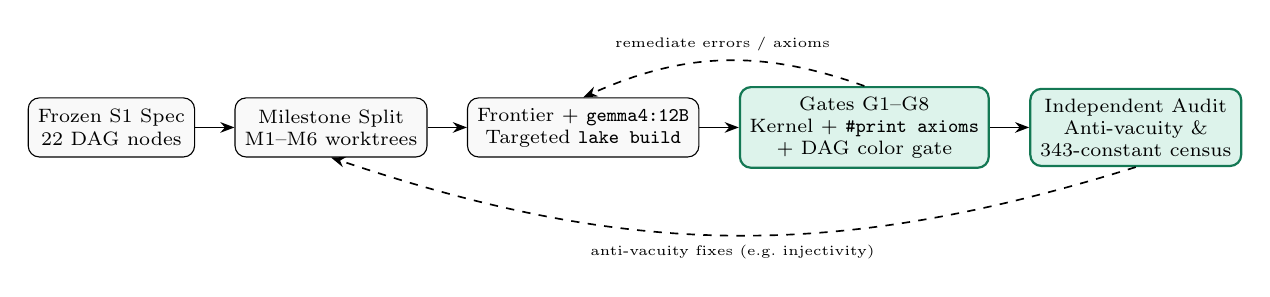
\begin{tikzpicture}[node distance=4.5mm and 5.0mm, every node/.style={font=\scriptsize},
  box/.style={draw,rounded corners,align=center,inner sep=3.5pt,minimum height=7.5mm,fill=gray!5},
  gate/.style={draw,rounded corners,align=center,inner sep=3.5pt,minimum height=7.5mm,fill=bpgreen!15,
               draw=bpgreen!70!black,thick},
  arr/.style={-{Stealth[length=1.8mm]},semithick}]
\node[box] (bp) {Frozen S1 Spec\\\NTotalNodes{} DAG nodes};
\node[box,right=of bp] (orch) {Milestone Split\\M1--M6 worktrees};
\node[box,right=of orch] (sub) {Frontier + \code{gemma4:12B}\\Targeted \code{lake build}};
\node[gate,right=of sub] (ver) {Gates G1--G8\\Kernel + \code{\#print axioms}\\+ DAG color gate};
\node[gate,right=of ver] (san) {Independent Audit\\Anti-vacuity \&\\343-constant census};
\draw[arr] (bp)--(orch);
\draw[arr] (orch)--(sub);
\draw[arr] (sub)--(ver);
\draw[arr] (ver)--(san);
\draw[arr,dashed] (ver.north) to[bend right=22] node[above,font=\tiny]{remediate errors / axioms} (sub.north);
\draw[arr,dashed] (san.south) to[bend left=18] node[below,font=\tiny]{anti-vacuity fixes (e.g.\ injectivity)} (orch.south);
\end{tikzpicture}%
}
\caption{The multi-agent Lean~4 + \code{leanblueprint} engineering and verification pipeline.}
\label{fig:pipeline}
\end{figure}

\paragraph{1. Frozen Specification and Anti-Vacuity Review.}
All 89 interface declarations were frozen at Gate~S1 (\code{gate-s1-frozen}) before proof work began,
catching and fixing a potential constant-0 collapse in \code{TM0Code.exists\_relabeling}.

\paragraph{2. Tiered Proving and Eight-Gate Verification.}
Routine T0 rewrite lemmas (26/45 attempted) were discharged by local \code{gemma4:12B} with
compiler-in-the-loop provenance tracking, while frontier models proved all headline theorems across
milestones M1--M6 under Gates G1--G8.

\begin{thebibliography}{99}\footnotesize\sloppy
\setlength{\itemsep}{1pt}
\bibitem{Lean4} L.~de Moura, S.~Ullrich, The Lean~4 theorem prover and programming language,
  \emph{Proc.\ CADE-28}, LNCS \textbf{12699} (2021), 625--635.
\bibitem{mathlib} The mathlib Community, The Lean mathematical library, \emph{Proc.\ CPP 2020}, 367--381.
\bibitem{TaoPFR} T.~Tao, Formalizing the proof of PFR in Lean4 using Blueprint: a short tour, 2023.
\end{thebibliography}

\newpage
\appendix
\section{Blueprint Dependency Graph}\label{app:graph}

\begin{center}
\vspace{0.5em}
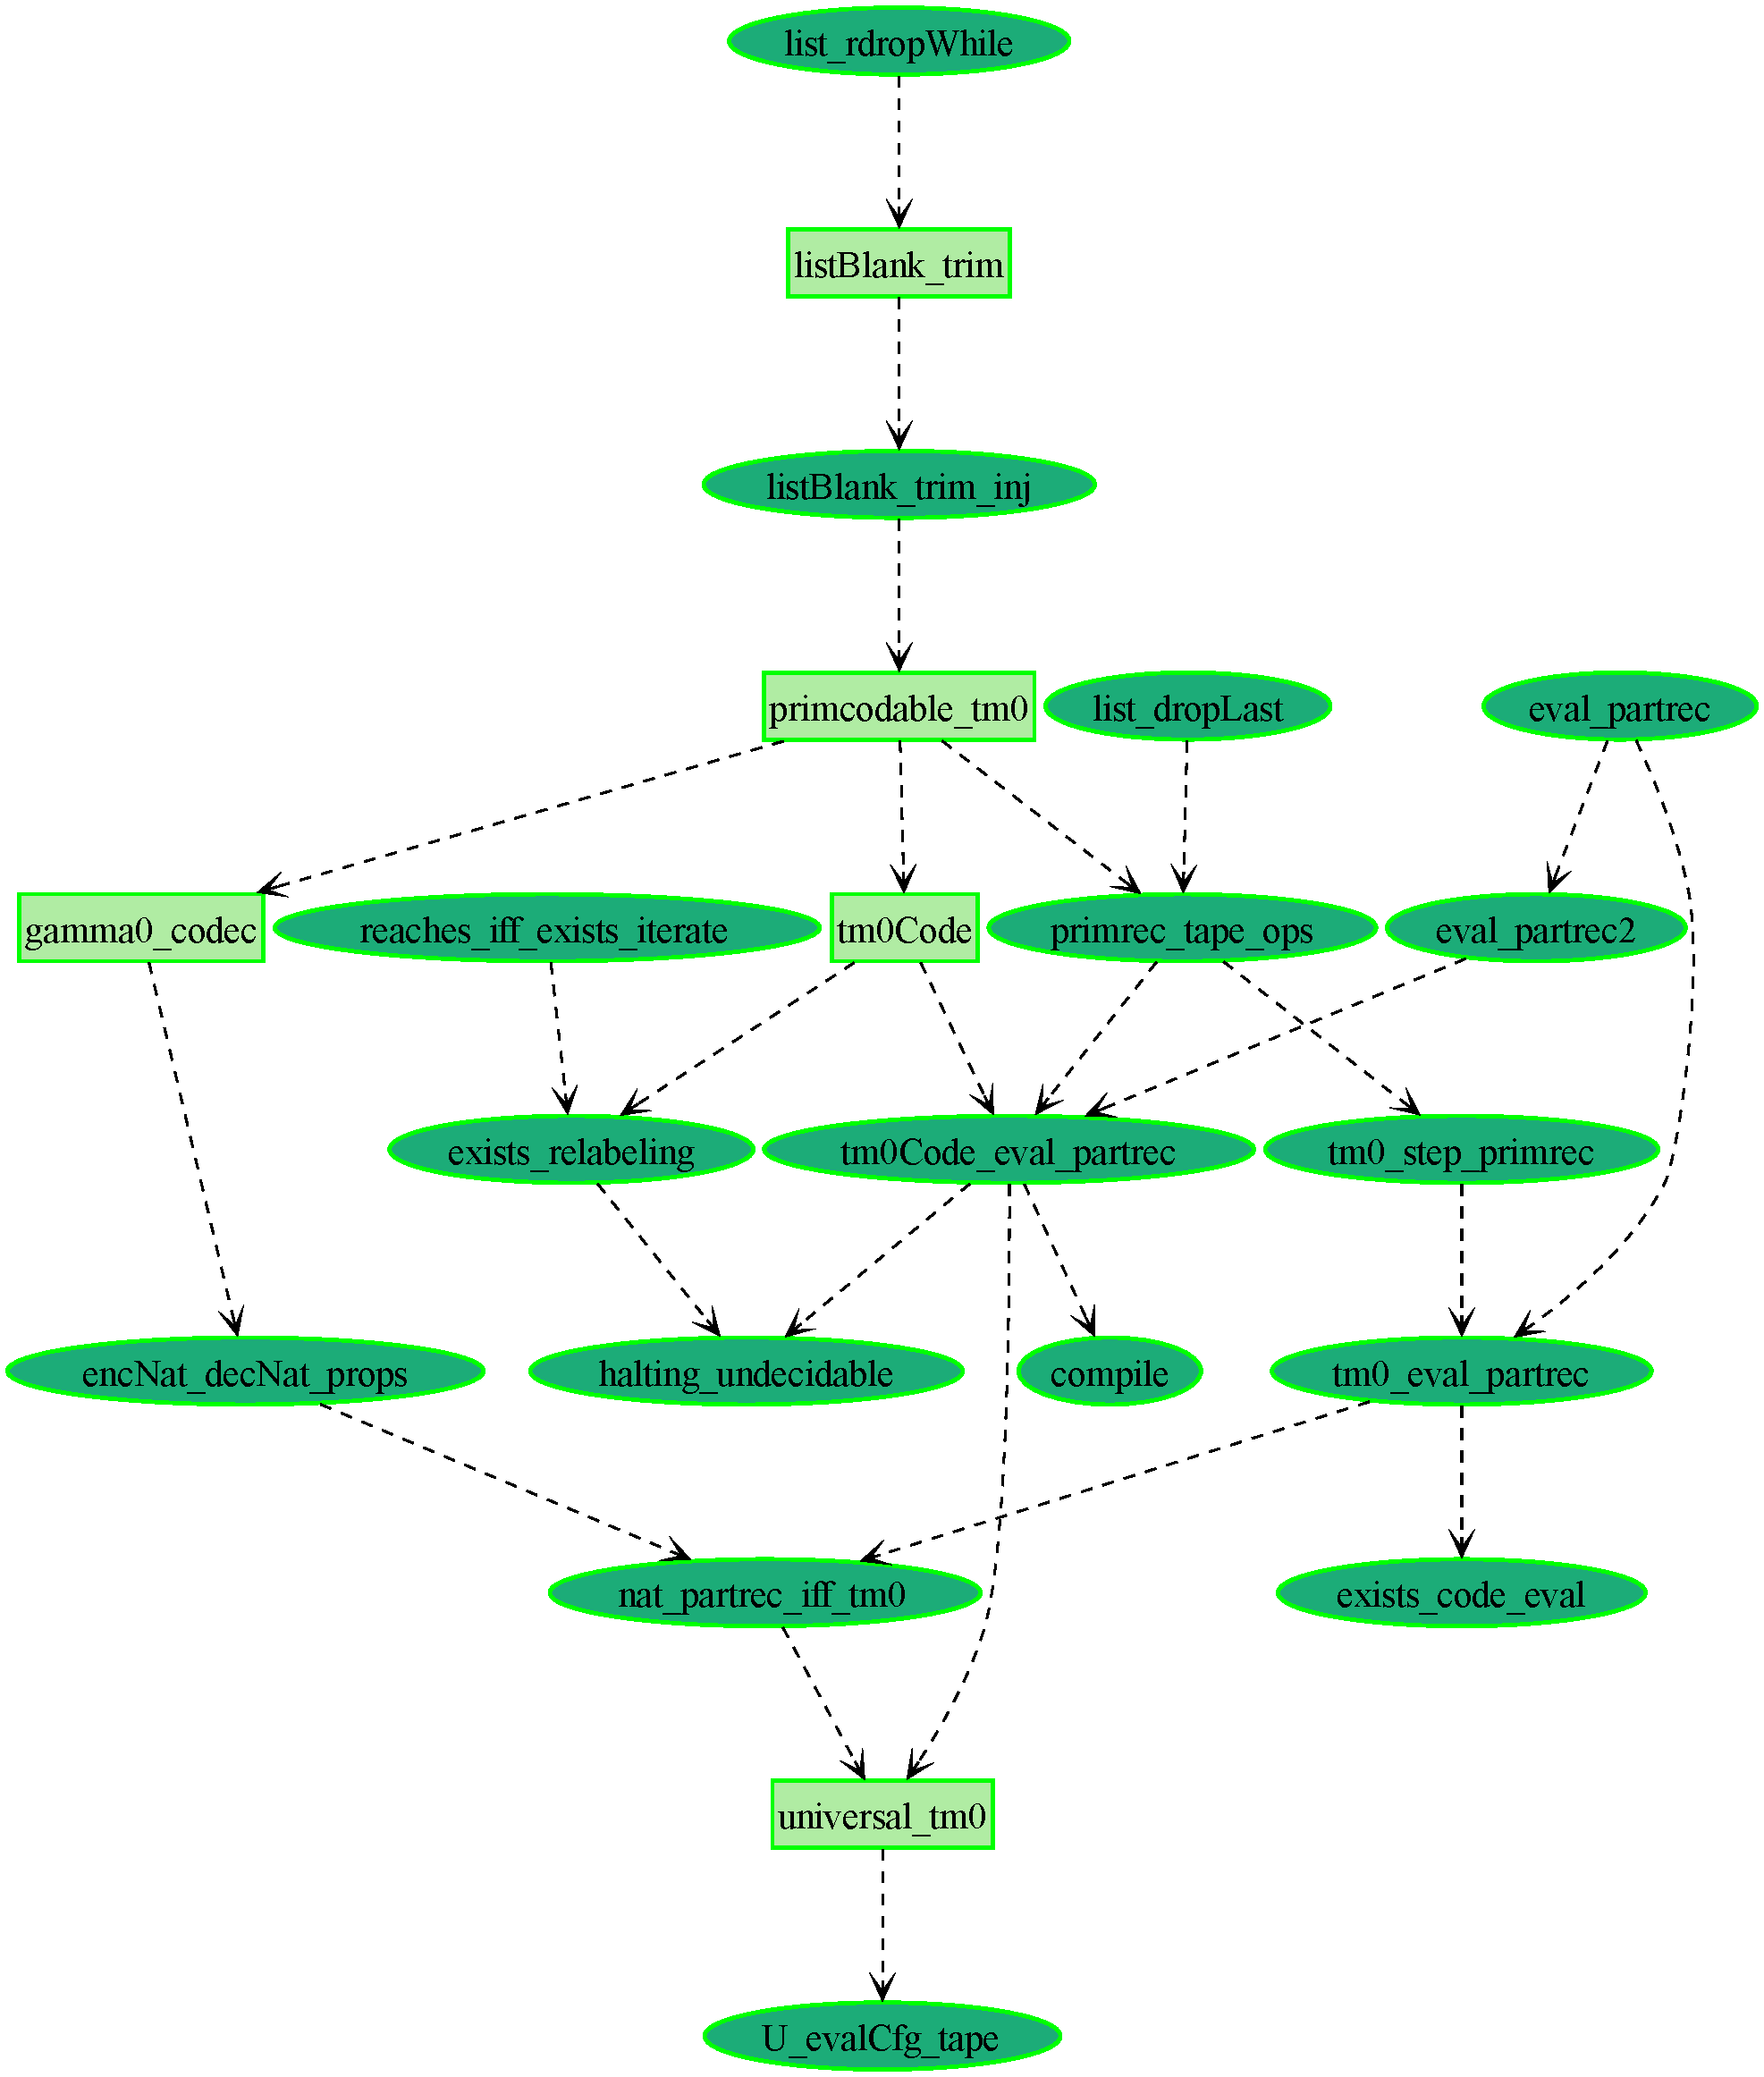
\includegraphics[width=\linewidth,height=0.80\textheight,keepaspectratio]{blueprint_dep_graph.pdf}
\end{center}
\vspace{0.5em}
\noindent\footnotesize\sloppy
\textbf{Figure A.1: Complete \code{leanblueprint} Dependency Graph (Portrait View).}
Generated from \code{blueprint/src/content.tex} via \code{build\_dep\_graph.py}
(interactive HTML version at \code{blueprint/web/dep\_graph\_document.html}).
Arrows point from each foundational definition or lemma to the downstream theorems that depend on it.
\textbf{Node shapes and colors:}
\textbf{Rectangles (\NDefNodes{} nodes, green \code{\#B0ECA3}):} Formalized mathematical definitions.
\textbf{Ellipses (\NProvedNodes{} nodes, dark green \code{\#1CAC78}):} Fully machine-checked theorems
and lemmas compiling with \code{0 sorryAx} and standard Lean~4 axioms across the entire dependency
closure.
\textbf{Unproved nodes:} $0$ light green (\code{\#9CEC8B}), $0$ light blue (\code{\#A3D6FF}).\par

\end{document}
